\documentclass[10pt]{beamer}

\usepackage[utf8]{inputenc}
\usepackage[T1]{fontenc}
\usepackage{amsmath,amssymb, mathrsfs}
\usepackage{dsfont}\let\mathbb\mathds
\usepackage[english]{babel}
\usepackage[all]{xy}
\usepackage{tikz-cd}
\usetikzlibrary{calc}
\usepackage{pgfplots}  

\institute{IBM Research Zurich\\ Université de Rennes 1}
\title{On Oriented Supersingular Isogeny Diffie Hellman}
\author{Pierrick Dartois \\ Under the supervision of Luca De Feo}
\titlegraphic{
\includegraphics[width=3.5cm]{logo_IBM.png}\hspace*{1.75cm}~%
   
\includegraphics[width=3.5cm]{logo_Rennes1.jpg}
}

\date{September 1 2021}

%\AtBeginSection[]
   %{
   %\begin{frame}
   %\tableofcontents[currentsection]
   %\end{frame}
%}

\usepackage{graphicx} 

\usetheme{Warsaw}

\usepackage{mathtools}

%\theoremstyle{definition}
%\newtheorem{definition}{Definition}

\theoremstyle{plain}
\newtheorem{proposition}{Proposition}
%\newtheorem{lemma}{Lemma}
%\newtheorem{corollary}{Corollary}
%\newtheorem{theorem}{Theorem}

\theoremstyle{definition}
\newtheorem{remark}{Remark}
%\newtheorem{example}{Example}

\usepackage{pgf,tikz}
\usetikzlibrary{arrows}

%To set line spacing
\usepackage{setspace}
% To cross text
\usepackage{ulem}

%macros
\newcommand{\ie}{\emph{i.e.}\ }
\newcommand{\eg}{\emph{e.g.}\ }
\newcommand{\N}{\mathbb{N}}
\newcommand{\Z}{\mathbb{Z}}
\newcommand{\Q}{\mathbb{Q}}
\newcommand{\R}{\mathbb{R}}
\newcommand{\C}{\mathbb{C}}
\newcommand{\K}{\mathbb{K}}
\newcommand{\F}{\mathbb{F}}
\newcommand{\Hc}{\mathbb{H}}
\newcommand{\Lc}{\mathbb{L}}
\newcommand{\M}{\mathbb{M}}
\newcommand{\Pc}{\mathbb{P}}
\newcommand{\A}{\mathbb{A}}
\newcommand{\B}{\mathbb{B}}
\newcommand{\E}{\mathbb{E}}
\newcommand{\V}{\mathbb{V}}
\newcommand{\m}[1]{\mathcal{#1}}
\newcommand{\mA}{\mathcal{A}}
\newcommand{\mB}{\mathcal{B}}
\newcommand{\mC}{\mathcal{C}}
\newcommand{\mP}{\mathcal{P}}
\newcommand{\mK}{\mathcal{K}}
\newcommand{\mL}{\mathcal{L}}
\newcommand{\mE}{\mathcal{E}}
\newcommand{\mD}{\mathcal{D}}
\newcommand{\mF}{\mathcal{F}}
\newcommand{\mO}{\mathcal{O}}
\DeclareMathOperator{\im}{im}
%\renewcommand{\ker}{\mbox{ker}}
%\renewcommand{\dim}{\mbox{dim}}
%\renewcommand{\deg}{\mbox{deg}}
\renewcommand{\i}[2]{\left\llbracket #1~;~#2\right\rrbracket}
\renewcommand{\(}{\left(}
\renewcommand{\)}{\right)}
\renewcommand{\P}{\mathbb{P}}
%commandes de Quentin
%\newcommand{\F}[1]{\mathbb{F}_{#1}}
\newcommand{\Fp}[1]{\mathbb{F}_{p^{#1}}}
\newcommand{\db}[1]{\mathbb{#1}}
\newcommand{\id}{\mbox{id}}
\newcommand{\mf}[1]{\mathfrak{#1}}
\newcommand{\mfm}{\mathfrak{m}}
\newcommand{\mfn}{\mathfrak{n}}
\newcommand{\mfp}{\mathfrak{p}}
\newcommand{\mfq}{\mathfrak{q}}
\DeclareMathOperator{\Spec}{Spec}
\DeclareMathOperator{\Proj}{Proj}
\DeclareMathOperator{\Hom}{Hom}
\DeclareMathOperator{\End}{End}
\DeclareMathOperator{\Aut}{Aut}
\DeclareMathOperator{\Tr}{Tr}
\DeclareMathOperator{\disc}{disc}
\DeclareMathOperator{\Cl}{Cl}
\let\SS\relax
\DeclareMathOperator{\SS}{SS}
\DeclareMathOperator{\Ell}{Ell}
%\DeclareMathOperator{\mod}{mod}
\DeclareMathOperator{\Gal}{Gal}
\DeclareMathOperator{\nrd}{nrd}
\DeclareMathOperator{\Vol}{Vol}
\DeclareMathOperator{\Covol}{Covol}
\DeclareMathOperator{\lcm}{lcm}
\DeclareMathOperator{\ProjEval}{ProjEval}
\DeclareMathOperator{\Char}{char}%\char already taken
\DeclareMathOperator{\DL}{DL}
\DeclareMathOperator{\argmax}{argmax}

\newcommand{\leftmapsto}{\leftarrow\!\shortmid}
\newcommand{\longleftmapsto}{\longleftarrow\!\shortmid}
\renewcommand{\vec}[1]{\mathbf{#1}}


\begin{document}

\begin{frame}
\titlepage
\end{frame}

\begin{frame}
\tableofcontents
\end{frame}

\section{Introduction}

\subsection{Presentation of IBM Research}

\begin{frame}
% 3000 poeple in 12 countries 
\textbf{Key research areas in IBM Research}

\begin{columns}[t]
\column{.5\textwidth}
\begin{figure}
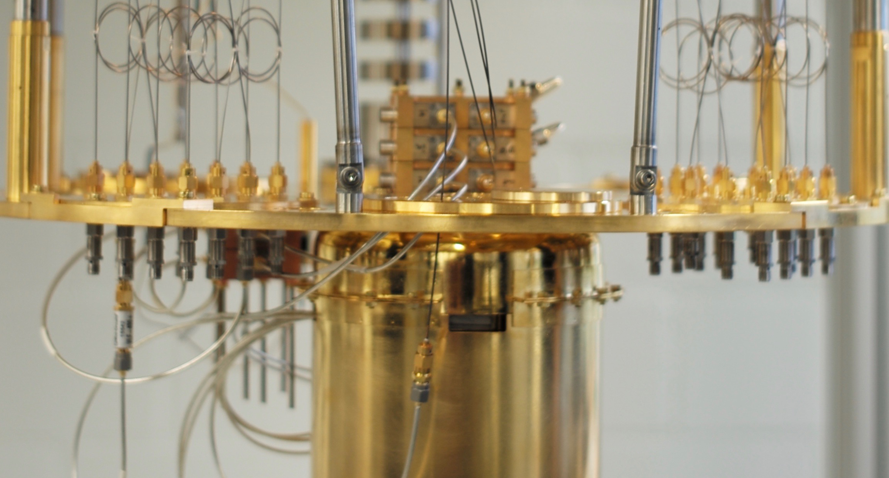
\includegraphics[width=3.5cm]
{science_and_technology.png} 

Science and Technology

\vspace{0.1cm}

{\setstretch{0.5} {\footnotesize Quantum computing, nanotechnologies, semi-conductors, electronics,  green technologies...}\\}
\vspace{0.3cm}


\includegraphics[width=3.5cm]
{security.jpg} 

Security

\vspace{0.1cm}

{\setstretch{0.5} {\footnotesize Post-quantum cryptography, blockchain, cybersecurity, identity and data governance...}\\}
\end{figure}


\column{.5\textwidth}

\begin{figure}

\includegraphics[width=3.5cm]
{cloud_and_AI.png} 

Cloud and AI

\vspace{0.1cm}

{\setstretch{0.5}{\footnotesize Machine learning, hardware technologies for storage, memory and processing in the cloud...}\\}

\vspace{0.3cm}

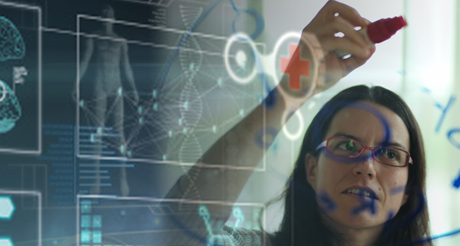
\includegraphics[width=3.5cm]
{cognitive_computing.jpg}

Cognitive computing

\vspace{0.1cm}

{\setstretch{0.5}{\footnotesize Computational biology and medicine, supercomputing, predictive maintenance...}\\}
\end{figure}
\end{columns}

\end{frame}

\subsection{Contextualization of OSIDH}

\subsubsection{Post quantum and isogeny based cryptography}

\begin{frame}
\textbf{Quantum computers are a threat to current cryptography}

\begin{itemize}
\item Shor's algorithm (1995) can compute discrete logarithms and factor integers on a quantum computer.

\item All current public key cryptography based on these problems may become unsafe (\sout{RSA} and \sout{El Gamal}).
\end{itemize}

\begin{columns}[t]
\column{.3\textwidth}

\begin{figure}
\includegraphics[width=3cm]{quantum_computer.png} 

\end{figure}


\column{.7\textwidth}

\begin{figure}
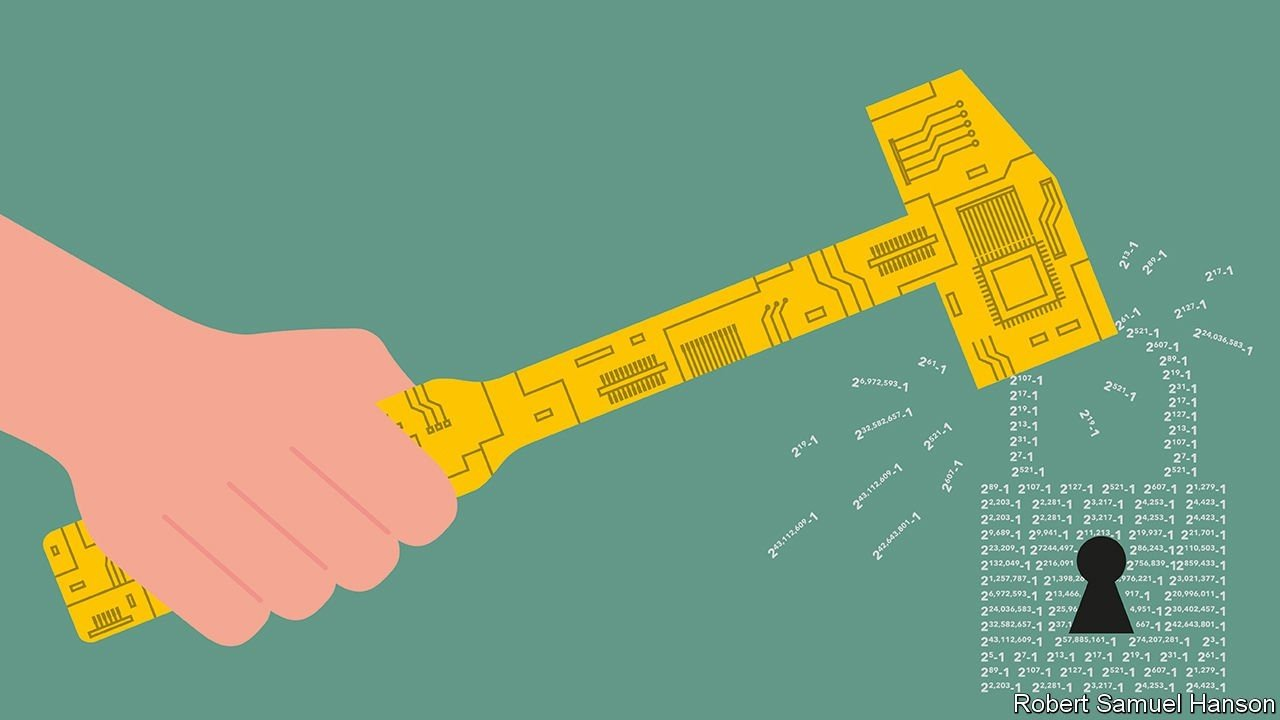
\includegraphics[width=6cm]{hammer.jpeg} 
\end{figure}

\end{columns}

\end{frame}



\begin{frame}
\textbf{Isogeny based cryptography in the NIST competition}


\begin{figure}
\begin{columns}[t]
\column{.5\textwidth}


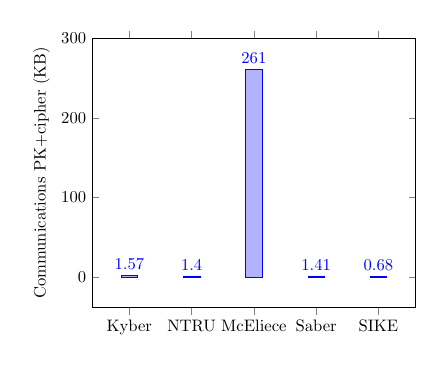
\begin{tikzpicture}[scale=0.6]
  
\begin{axis}  
[  
    ybar,  
    enlargelimits=0.15,  
    ylabel={Communications PK+cipher (KB)}, % the ylabel must precede a # symbol.  
    %xlabel={},  
    symbolic x coords={Kyber, NTRU, McEliece, Saber, SIKE}, % these are the specification of coordinates on the x-axis.  
    xtick=data,  
     nodes near coords, % this command is used to mention the y-axis points on the top of the particular bar.  
    nodes near coords align={vertical},  
    ]  
\addplot coordinates {(Kyber,1.568) (NTRU,1.398) (McEliece,261) (Saber,1.408) (SIKE,0.676) };  
  
\end{axis}  
\end{tikzpicture} 
\column{.5\textwidth}


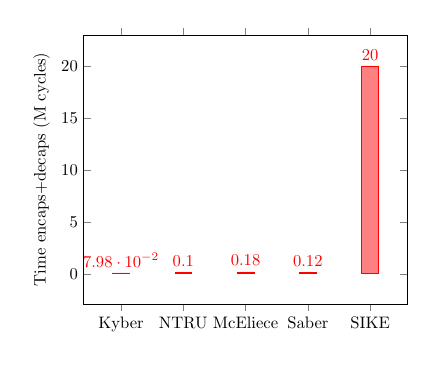
\begin{tikzpicture}[scale=0.6]
  
\begin{axis}  
[  
    ybar,  
    enlargelimits=0.15,  
    ylabel={Time encaps+decaps (M cycles)}, % the ylabel must precede a # symbol.  
    %xlabel={},  
    symbolic x coords={Kyber, NTRU, McEliece, Saber, SIKE}, % these are the specification of coordinates on the x-axis.  
    xtick=data,  
     nodes near coords, % this command is used to mention the y-axis points on the top of the particular bar.  
    nodes near coords align={vertical},  
    ]  
\addplot[color=red,fill=red!50] coordinates {(Kyber,0.079772) (NTRU,0.101357) (McEliece,0.179095) (Saber,0.124) (SIKE,20) };  
  
\end{axis}  
\end{tikzpicture}


\end{columns}

\caption{Total communication size (public key and cipher) and time performance (encapsulation and decapsulation) of 5 NIST round 3 key encapsulation mechanisms candidates.}
\end{figure}

\end{frame}

\subsubsection{Cryptographic group actions and Diffie-Hellman key-exchange}


\begin{frame}
\textbf{Cryptographic group action}

\vspace{0.5cm}

\begin{itemize}
\item $G$: a group.
\item $X$: a set ($|X|=|G|$).
\pause 
\item $\cdot : G\times X\longrightarrow X$ a \emph{transitive} and \emph{faithful} group action:
\[\forall x,y\in X, \exists g\in G, \quad g\cdot x=y \quad (\mbox{transitivity})\]
\[\forall x\in X,  g\in G, \quad g\cdot x=x \Longrightarrow g=e \quad (\mbox{faithfulness})\]
\pause
\item Group action easy to compute.
\item \emph{One way} group action: hard to guess $g\in G$, with the knowledge of $x\in X$ and $g\cdot x$.
\end{itemize}

\end{frame}

\begin{frame}
\textbf{Diffie-Hellman key exchange}

\vspace{0.5cm}

\begin{itemize}
\item Public parameter: $x_0\in X$.
\item Alice's secret: $g\in G$.
\item Bob's secret: $h\in G$.
\end{itemize}

\pause

\begin{columns}[t]
\column{.4\textwidth}


\[\xymatrix{
x_0 \ar[d]^{h} \ar[r]^{g} & g\cdot x_0 \ar[d]^{h} \\
h\cdot x_0 \ar[r]^{g} & (gh)\cdot x_0
}\]


\column{.6\textwidth}

\begin{tikzpicture}[scale=1]

  \tikzstyle{every node}=[transform shape];

  % Alice
  \node (Alice) at (0,0) {
\includegraphics[height=2cm]{Alice.jpg}};
  \node (label) at (0,-1.5) {Alice};
  
  % Bob
  \node (Bob) at (4,0) {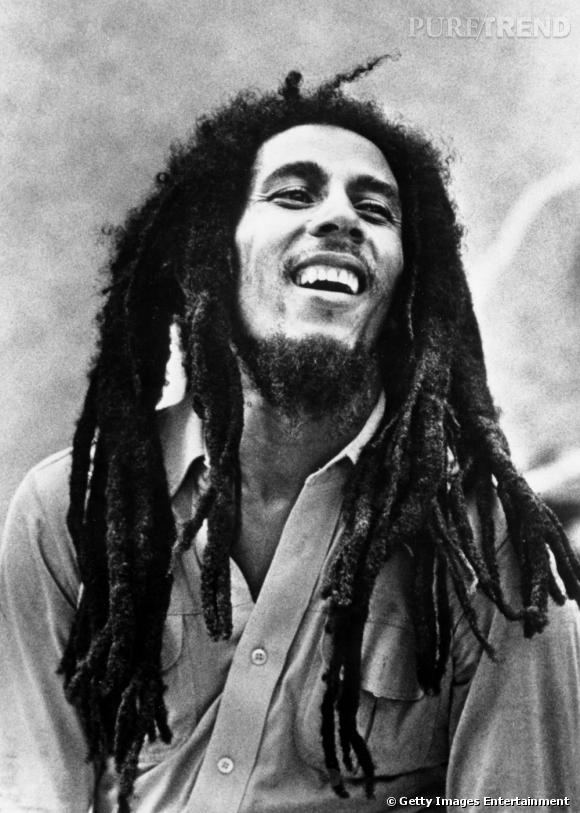
\includegraphics[height=2cm]{Bob.jpg}};
  \node (label) at (4,-1.5) {Bob};

% Messages
\draw[->,thick] ($(Alice)+(0.5,0.25)$) -- ($(Bob)+(-0.75,0.25)$) node [pos=0.5,above,font=\footnotesize] {$g\cdot x_0$};
\draw[->,thick] ($(Bob)+(-0.75,-0.25)$) -- ($(Alice)+(0.5,-0.25)$) node [pos=0.5,above,font=\footnotesize] {$h\cdot x_0$};

\end{tikzpicture}

\end{columns}

\end{frame}
%Show cryptographic group action, Couveignes cryptosystem, CSIDH, OSIDH.

\section{Introduction to OSIDH}

\subsection{Orientations}

\begin{frame}
\textbf{Oriented elliptic curves}

\vspace{0.5cm}

\begin{itemize}
\item $K$: quadratic imaginary field.
\item $\mO$: order of $K$.
\item $E/\F_q$: elliptic curve.
\end{itemize}

\begin{definition}
A $K$-\emph{orientation} of $E$ is an embedding: 
\[\iota : K\hookrightarrow \End(E)\otimes_\Z\Q.\]

$(E, \iota)$ is an $\mO$-\emph{orientation} if $\iota(\mO)\subseteq \End(E)$.  

It is \emph{primitive} if $\iota(\mO)=\End(E)\cap\iota(K)$.
\end{definition}

\pause

\begin{itemize}
\item If $E$ is ordinary, then $\iota(K)=\End(E)\otimes_\Z\Q$. Not very interesting.

\pause
\item If $E$ is supersingular, $\End(E)$ is a maximal order in a quaternion algebra: infinitely many possible orientations.
\end{itemize}

\end{frame}

\begin{frame}
\textbf{$K$-oriented isogenies}

\vspace{0.5cm}

\begin{itemize}
\item $(E, \iota)$ is a $K$-oriented elliptic curve. 
\item $\varphi : E\longrightarrow F$ is an isogeny.
\item We define a $K$-orientation $\varphi_*(\iota)$ on $F$ by:
\[\forall \alpha\in K,  \quad \varphi_*(\iota)(\alpha)=\frac{1}{\deg(\varphi)}\varphi\circ \iota(\alpha)\circ \widehat{\varphi}.\]
\end{itemize}

\begin{definition}
Let $(E, \iota_E)$ and $(F,\iota_F)$ be two $K$-oriented elliptic curves.  

An isogeny $\varphi : E\longrightarrow F$ is $K$-\emph{oriented} if $\varphi_*(\iota_E)=\iota_F$.  

We denote this by $\varphi : (E, \iota_E)\longrightarrow(F,\iota_F)$.
\end{definition}

\end{frame}

\begin{frame}
\textbf{Ascending, horizontal, descending $K$-oriented isogenies}

\vspace{0.5cm}

\begin{itemize}
\item $\varphi : (E, \iota_E)\longrightarrow(F,\iota_F)$, a $K$-oriented isogeny.
\item $\mO:=\iota_E^{-1}(\End(E))$.
\item $\mO':=\iota_F^{-1}(\End(F))$.

\pause
\item If $\mO\subseteq\mO'$, then $\varphi$ is \emph{ascending}.
\item If $\mO=\mO'$, then $\varphi$ is \emph{horizontal}.
\item If $\mO\supseteq\mO'$, then $\varphi$ is \emph{descending}.
\end{itemize}

\pause

\begin{proposition}
If $\ell:=\deg(\varphi)$ is prime, then: 
\begin{description}
\item[(i)] $\varphi$ is always ascending, horizontal or descending.
\item[(ii)] If $\varphi$ is ascending, then $[\mO':\mO]=\ell$.
\item[(iii)] If $\varphi$ is descending, then $[\mO:\mO']=\ell$.
\end{description}

\end{proposition}

\end{frame}

\subsection{Oriented supersingular isogeny graphs}

\begin{frame}
\textbf{$K$-oriented supersingular $\ell$-isogeny graphs}
\vspace{0.5cm}
\begin{itemize}
\item $\ell$ and $p$ distinct prime numbers.
\item $p$ does not split in $K$.
\item \textbf{Vertices:} $K$-oriented supersingular elliptic curves defined over $\F_{p^2}$ up to $K$-oriented isomorphism.
\item \textbf{Edges:} $K$-oriented isogenies of degree $\ell$.
\end{itemize}

\end{frame}

\begin{frame}

\textbf{The volcano structure}

\vspace{0.5cm}

\begin{proposition}[Kohel]
Let $(E,\iota)$ be a supersingular primitively $\mO$-oriented elliptic curve and $\Delta_K:=\disc(K)$. Then:

\begin{description}
\item[(i)] If $\ell\nmid [\mO_K:\mO]$, among the $\ell$-isogenies with origin $(E,\iota)$:
\begin{itemize}
\item $1+\(\frac{\Delta_K}{\ell}\)$ are horizontal;
\item $1/[\mO^\times:(\Z+\ell\mO)^\times]\(\ell-\(\frac{\Delta_K}{\ell}\)\)$ are descending;
\item none of them are ascending.
\end{itemize}

\item[(ii)] If $\ell|[\mO_K:\mO]$, among the $\ell$-isogenies with origin $(E,\iota)$:
\begin{itemize}
\item none are horizontal;
\item $\ell$ are descending;
\item one of them are ascending.
\end{itemize}
\end{description}
\end{proposition}

\textbf{N.B.} These isogenies are considered up to $K$-oriented isomorphism.

\end{frame}

\begin{frame}

\textbf{Example:} $K=\Q(i)$, $\ell=2$, $p=79$,  $\F_{79^2}=\F_{79}[a]$ with $a^2-a+3=0$.

\begin{figure}[h!]
\centering

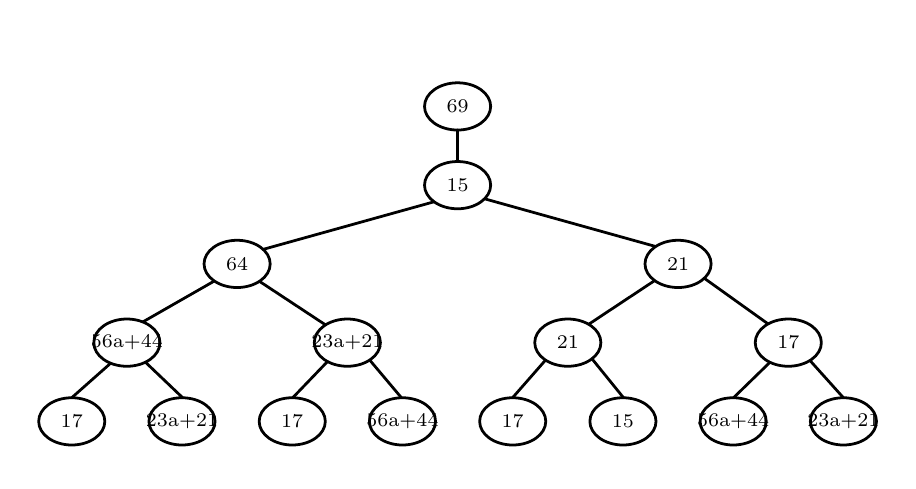
\begin{tikzpicture}[line cap=round,line join=round,>=triangle 45,x=1.4cm,y=1cm,scale=1]
\clip(-3.9,-4.5) rectangle (3.9,1);
\draw [line width=1pt] (3.5,-4) circle (0.3);
\draw [line width=1pt] (0,0) circle (0.3);
\draw [line width=1pt] (-1.5,-4) circle (0.3);
\draw [line width=1pt] (-3.5,-4) circle (0.3);
\draw [line width=1pt] (0.5,-4) circle (0.3);
\draw [line width=1pt] (2,-2) circle (0.3);
\draw [line width=1pt] (1.5,-4) circle (0.3);
\draw [line width=1pt] (-0.5,-4) circle (0.3);
\draw [line width=1pt] (-2.5,-4) circle (0.3);
\draw [line width=1pt] (-1,-3) circle (0.3);
\draw [line width=1pt] (-3,-3) circle (0.3);
\draw [line width=1pt] (0,-1) circle (0.3);
\draw [line width=1pt] (-2,-2) circle (0.3);
\draw [line width=1pt] (3,-3) circle (0.3);
\draw [line width=1pt] (1,-3) circle (0.3);
\draw [line width=1pt] (2.5,-4) circle (0.3);
\draw [line width=1pt] (0,-0.3)-- (0,-0.7);
\draw [line width=1pt] (-0.21322943610478404,-1.2110289259282618)-- (-1.763489092966821,-1.8154394656099442);
\draw [line width=1pt] (-1.7974860543853213,-2.2213325593571245)-- (-1.1980343823186057,-2.774650530465039);
\draw [line width=1pt] (-2.2067876385720067,-2.217345054081783)-- (-2.855544073501337,-2.7370694287470303);
\draw [line width=1pt] (-2.8316599983612933,-3.248317626938323)-- (-2.493627811564869,-3.700067682277239);
\draw [line width=1pt] (-3.1470895453233143,-3.261466375766714)-- (-3.5006593390669343,-3.70000072454755);
\draw [line width=1pt] (-1.18,-3.24)-- (-1.4957111195996629,-3.7000306590584437);
\draw [line width=1pt] (-0.797179438826777,-3.2210516228517196)-- (-0.5091578288571417,-3.70013980895987);
\draw [line width=1pt] (0.24489723766178567,-1.1732782242107382)-- (1.7970406198298907,-1.7790758274860692);
\draw [line width=1pt] (1.7876443158207822,-2.2119081484907466)-- (1.1890212652361931,-2.7670387128973815);
\draw [line width=1pt] (0.7978265785504022,-3.2216436501670267)-- (0.49846155869074266,-3.700003944695371);
\draw [line width=1pt] (1.2190320192368846,-3.2049999379244123)-- (1.5054935841881036,-3.700050303329428);
\draw [line width=1pt] (2.2379689093048514,-2.18267675879613)-- (2.8168942423162138,-2.7623610269693826);
\draw [line width=1pt] (3.1965297683390395,-3.2266628557055688)-- (3.5002064693248105,-3.700000071049312);
\draw [line width=1pt] (2.833538103582579,-3.249580522158913)-- (2.5028570132903156,-3.7000136045167067);
\begin{scriptsize}
\draw[color=black] (3.5,-4) node {23a+21};
\draw[color=black] (0,0) node {69};
\draw[color=black] (-1.5,-4) node {17};
\draw[color=black] (-3.5,-4) node {17};
\draw[color=black] (0.5,-4) node {17};
\draw[color=black] (2,-2) node {21};
\draw[color=black] (1.5,-4) node {15};
\draw[color=black] (-0.5,-4) node {56a+44};
\draw[color=black] (-2.5,-4) node {23a+21};
\draw[color=black] (-1,-3) node {23a+21};
\draw[color=black] (-3,-3) node {56a+44};
\draw[color=black] (0,-1) node {15};
\draw[color=black] (-2,-2) node {64};
\draw[color=black] (3,-3) node {17};
\draw[color=black] (1,-3) node {21};
\draw[color=black] (2.5,-4) node {56a+44};
\end{scriptsize}
\end{tikzpicture}
\end{figure}

\end{frame}

\begin{frame}

\textbf{Example:} $K=\Q(i)$, $\ell=2$, $p=79$,  $\F_{79^2}=\F_{79}[a]$ with $a^2-a+3=0$.

\vspace{0.3cm}

\textbf{The graph refolds!}

\begin{figure}[h!]
\centering

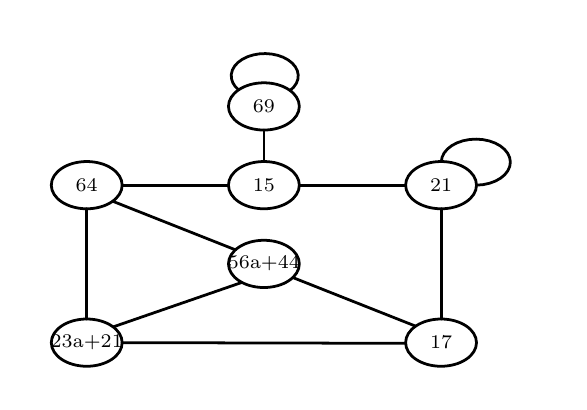
\begin{tikzpicture}[line cap=round,line join=round,>=triangle 45,x=1.5cm,y=1cm,scale=1]
\clip(-2,-3.5) rectangle (2.5,1);
\draw [line width=1pt] (0,0) circle (0.3);
\draw [line width=1pt] (0,-1) circle (0.3);
\draw [line width=1pt] (1.5,-1) circle (0.3);
\draw [line width=1pt] (-1.5,-1) circle (0.3);
\draw [line width=1pt] (1.5,-3) circle (0.3);
\draw [line width=1pt] (-1.5,-3) circle (0.3);
\draw [line width=1pt] (0,-2) circle (0.3);
\draw [line width=1pt] (0,-0.3)-- (0,-0.7);
\draw [line width=1pt] (0.3,-1)-- (1.2,-1);
\draw [line width=1pt] (1.5022058227240238,-1.2999918904672427)-- (1.5022058227240238,-2.7000081095327575);
\draw [line width=1pt] (1.2001241400766958,-3.0086295211488694)-- (-1.2,-3);
\draw [line width=1pt] (-1.5021428024802257,-1.2999923472316097)-- (-1.5021428024802257,-2.7000076527683903);
\draw [line width=1pt] (-1.2,-1)-- (-0.3,-1);
\draw [line width=1pt] (-1.2802410299272011,-1.2042204570373467)-- (-0.24099353148483596,-1.8213323818302058);
\draw [line width=1pt] (-0.18632449139731455,-2.235123762953752)-- (-1.2762572482543024,-2.80015210523685);
\draw [line width=1pt] (0.2449732494851846,-2.173170745325732)-- (1.2848736133624907,-2.79090519429625);
\draw [shift={(0.007090427603428667,0.3874717685141776)},line width=1pt]  plot[domain=-0.7124630393351774:3.8174613554669614,variable=\t]({1*0.2837279521520933*cos(\t r)+0*0.2837279521520933*sin(\t r)},{0*0.2837279521520933*cos(\t r)+1*0.2837279521520933*sin(\t r)});
\draw [shift={(1.7943119546152102,-0.7077247818460842)},line width=1pt]  plot[domain=-1.551337518465128:3.115189512445009,variable=\t]({1*0.2923305611926651*cos(\t r)+0*0.2923305611926651*sin(\t r)},{0*0.2923305611926651*cos(\t r)+1*0.2923305611926651*sin(\t r)});
\begin{scriptsize}
\draw[color=black] (0,0) node {69};
\draw[color=black] (0,-1) node {15};
\draw[color=black] (1.5,-1) node {21};
\draw[color=black] (-1.5,-1) node {64};
\draw[color=black] (1.5,-3) node {17};
\draw[color=black] (-1.5,-3) node {23a+21};
\draw[color=black] (0,-2) node {56a+44};
\end{scriptsize}
\end{tikzpicture}

\caption{Supersingular $2$-isogeny graph over $\F_{79^2}$.}
\end{figure}

\end{frame}

\begin{frame}
\textbf{Representing $K$-oriented elliptic curves by $j$-invariants}

\vspace{0.5cm}

\begin{itemize}
\item $\SS_K(p)$: set of $K$-oriented supersingular elliptic curves over $\F_{p^2}$ up to $K$-oriented isomomorphism.
\item $\SS(p)$: set of supersingular elliptic curves over $\F_{p^2}$ up to isomomorphism (supersingular $j$-invariants).
\item Unfortunatelly, the \emph{forgetful map}:
\[(E,\iota)\in\SS_K(p)\longmapsto E\in\SS(p)\]
is not injective.
\end{itemize}

\end{frame}

\begin{frame}
\textbf{Representing $K$-oriented elliptic curves by $j$-invariants}

\vspace{0.5cm}

\begin{itemize}
\item But we can restrict to $\mO$-orientations with $\disc(\mO)$ bounded.
\item $\SS_{\mO}(p)$: set of $\mO$-oriented supersingular elliptic curves over $\F_{p^2}$ up to $K$-oriented isomomorphism.
\end{itemize}

\begin{theorem}
If $p>|\disc(\mO)|$, then the forgetful map:
\[(E,\iota)\in\SS_{\mO}(p)\longmapsto E\in\SS(p)\]
is injective.
\end{theorem}

\end{frame}

\subsection{The ideal class group action}

\begin{frame}
\textbf{The ideal class group action}

\vspace{0.5cm}

\begin{itemize}
\item $\SS_{\mO}^{pr}(p)$: set of \textbf{primitively} $\mO$-oriented supersingular elliptic curves over $\F_{p^2}$ up to $K$-oriented isomorphism.
\item We define a group action:
\[\Cl(\mO)\times\SS_{\mO}^{pr}(p)\longrightarrow \SS_{\mO}^{pr}(p)\]
\item If $(E,\iota)\in \SS_{\mO}^{pr}(p)$ and $\mf{a}\subseteq\mO$ has norm prime to $p$, we consider:
\[\varphi_{\mf{a}}:E\longrightarrow E/E[\mf{a}]\]
with:
\[\ker(\varphi_{\mf{a}})=E[\mf{a}]:=\bigcap_{\alpha\in\mf{a}}\ker(\iota(\alpha))\]
\item We set:
\[[\mf{a}]\cdot (E,\iota):=(E/E[\mf{a}],(\varphi_{\mf{a}})_*(\iota))\]
\end{itemize}
\end{frame}

\begin{frame}
\textbf{The ideal class group action}

\vspace{0.5cm}

\begin{theorem}
The ideal class group action $\Cl(\mO)\times\SS_{\mO}^{pr}(p)\longrightarrow \SS_{\mO}^{pr}(p)$ is well-defined, \textbf{faithful} but \textbf{not transitive}. Actually, there are two orbits.
\end{theorem}

\vspace{0.5cm}

\pause

\textbf{To make it transitive:} restrict to the orbit of elliptic curves obtained by reduction mod $p$ of elliptic curves defined over a number field with complex multiplication by $\mO$. 

\end{frame}

\subsection{Chains and ladders}

\section{The OSIDH protocol}

\subsection{A broken naive Diffie Hellman protocol}

\subsection{Why is it broken?}

\subsection{A fixed Diffie Hellman protocol}

\section{Cryptanalysis of OSIDH}

\subsection{Recovering the chain with oriented endomorphisms}

\subsection{A lattice reduction to find oriented endomorphisms}

\subsection{Implementation of our attack}

\subsection{Countermeasures}

\section{Conclusion}

\end{document}